\documentclass[12pt,a4paper]{report}

% ── Packages ──────────────────────────────────────────────────────────────────
\usepackage[margin=1in]{geometry}
\usepackage{graphicx}
\usepackage{xcolor}
\usepackage{tikz}
\usetikzlibrary{shapes.geometric, arrows.meta, positioning, fit, backgrounds, calc}
\usepackage{booktabs}
\usepackage{array}
\usepackage{longtable}
\usepackage{hyperref}
\usepackage{enumitem}
\usepackage{fancyhdr}
\usepackage{titlesec}
\usepackage{setspace}
\usepackage[T1]{fontenc}
\usepackage[utf8]{inputenc}
\newcommand{\taka}{Tk.}
% \usepackage{microtype}
\usepackage{listings}
\usepackage{caption}
\usepackage{subcaption}
\usepackage{float}
\usepackage{multirow}
\usepackage{tabularx}
\usepackage{amssymb}
% \usepackage{mdframed}

% ── Colours ───────────────────────────────────────────────────────────────────
\definecolor{primary}{RGB}{8,107,79}
\definecolor{accent}{RGB}{225,67,80}
\definecolor{darkbg}{RGB}{17,24,39}
\definecolor{lightgray}{RGB}{243,244,246}
\definecolor{coolgray}{RGB}{107,114,128}
\definecolor{linkblue}{RGB}{37,99,235}
\definecolor{codebg}{RGB}{248,249,250}

% ── Hyperref setup ────────────────────────────────────────────────────────────
\hypersetup{
  colorlinks=true,
  linkcolor=primary,
  urlcolor=linkblue,
  citecolor=primary,
  pdfauthor={Shihab Shaharia, Abid Ahmed Angkon, Mahfuz Iqram Sunny},
  pdftitle={Expenser - Project Report},
}

% ── Header / Footer ───────────────────────────────────────────────────────────
\pagestyle{fancy}
\fancyhf{}
\fancyhead[L]{\small\textcolor{coolgray}{Expenser — Personal Finance Tracker}}
\fancyhead[R]{\small\textcolor{coolgray}{CSE474.3 · Southeast University}}
\fancyfoot[C]{\small\textcolor{coolgray}{\thepage}}
\renewcommand{\headrulewidth}{0.4pt}

% ── Section formatting ────────────────────────────────────────────────────────
\titleformat{\chapter}[display]
  {\normalfont\huge\bfseries\color{darkbg}}
  {\color{primary}\chaptertitlename\ \thechapter}{12pt}{\Huge}
\titlespacing*{\chapter}{0pt}{-10pt}{20pt}
\titleformat{\section}
  {\normalfont\Large\bfseries\color{darkbg}}{\thesection}{1em}{}
\titleformat{\subsection}
  {\normalfont\large\bfseries\color{darkbg}}{\thesubsection}{1em}{}
\titleformat{\subsubsection}
  {\normalfont\normalsize\bfseries\color{coolgray}}{\thesubsubsection}{1em}{}

% ── Listings (code) ───────────────────────────────────────────────────────────
\lstset{
  basicstyle=\ttfamily\small,
  backgroundcolor=\color{codebg},
  frame=single,
  rulecolor=\color{lightgray},
  breaklines=true,
  captionpos=b,
}

% ── TikZ styles ───────────────────────────────────────────────────────────────
\tikzset{
  entity/.style={rectangle, draw=primary, fill=primary!8, rounded corners=4pt,
                 minimum width=2.8cm, minimum height=0.7cm, font=\small\bfseries,
                 text=darkbg, align=center},
  attr/.style={rectangle, draw=gray!50, fill=white, rounded corners=2pt,
               minimum width=2.8cm, minimum height=0.55cm, font=\footnotesize,
               text=darkbg, align=left, inner sep=4pt},
  arrow/.style={-{Latex[length=3pt]}, gray!70, line width=0.6pt},
  box/.style={rectangle, draw=primary!40, fill=primary!5, rounded corners=6pt,
              minimum width=3cm, minimum height=1cm, font=\small\bfseries,
              text=darkbg, align=center},
  layer/.style={rectangle, draw=gray!40, fill=lightgray, rounded corners=4pt,
                font=\footnotesize\bfseries, text=coolgray, align=center},
}

% ─────────────────────────────────────────────────────────────────────────────
\begin{document}
\onehalfspacing

% ══════════════════════════════════════════════════════════════════════════════
%  COVER PAGE
% ══════════════════════════════════════════════════════════════════════════════
\begin{titlepage}
\thispagestyle{empty}
\centering

\vfill

{\LARGE\bfseries EXPENSER}\\[4pt]
{\large\itshape Personal Finance Tracker}\\[2pt]
{\small\itshape A Django-based Web Application for Income, Expense \& Budget Management}

\vfill

\noindent\rule{\linewidth}{0.6pt}

\vfill

{\large\bfseries Submitted By}\\[10pt]

\begin{tabular}{@{}lc@{}}
\toprule
\textbf{Student Name} & \textbf{Student ID} \\
\midrule
Shihab Shaharia    & 2023100010136 \\[2pt]
Abid Ahmed Angkon  & 2023200010039 \\[2pt]
Mahfuz Iqram Sunny & 2023200010034 \\
\bottomrule
\end{tabular}

\vfill

{\large\bfseries PROJECT REPORT}\\[6pt]
{\normalsize This Report Presented in Partial Fulfillment of the Course}\\[4pt]
{\normalsize\bfseries CSE474.3: Software Development and Project Management}\\[4pt]
{\normalsize in the Computer Science and Engineering Department}\\[8pt]
{\normalsize \textbf{Submitted To:} Md. Anower Perves (AP)}\\[2pt]
{\normalsize Lecturer, Department of CSE, Southeast University}

\vfill


\includegraphics[width=3.8cm]{seu_logo.png}\\[8pt]
{\Large\bfseries SOUTHEAST UNIVERSITY}\\[4pt]
{\normalsize Dhaka, Bangladesh}\\[3pt]
{\normalsize June 6, 2026}

\vfill

\noindent\rule{\linewidth}{0.6pt}

\end{titlepage}

% ══════════════════════════════════════════════════════════════════════════════
%  TABLE OF CONTENTS
% ══════════════════════════════════════════════════════════════════════════════
\tableofcontents
\newpage

% ══════════════════════════════════════════════════════════════════════════════
%  ABSTRACT
% ══════════════════════════════════════════════════════════════════════════════
\chapter*{Abstract}
\addcontentsline{toc}{chapter}{Abstract}

This report documents the design, development, and implementation of \textbf{Expenser}, a web-based personal finance management application built as part of the CSE474.3 Software Development and Project Management Lab at Southeast University.

Expenser allows registered users to record daily income and expense transactions, organise them by category and tag, set monthly spending budgets per category, and generate financial reports over flexible date ranges. Reports can also be exported as CSV files. The application is built using Python 3.12 and Django 5.2 on the backend, PostgreSQL 16 as the database, and Tailwind CSS for the frontend. It runs on a Linux virtual machine environment.

The project was developed by a team of three students using an Agile methodology. Work was split across two sprints: the first sprint covered the initial development of all features, and the second sprint focused on testing, bug fixing, and refining the application based on what we found after running everything together for the first time.

The source code is publicly available at:
\begin{center}
\url{https://github.com/shihabshaharia/expenser}
\end{center}

\newpage

% ══════════════════════════════════════════════════════════════════════════════
\chapter{Introduction}
% ══════════════════════════════════════════════════════════════════════════════

Expenser is a web-based personal finance management application developed as part of the CSE474.3 Software Development and Project Management Lab course at Southeast University. The main idea behind this project was to build something useful while learning Django properly. We wanted to make a simple tool where a user can log their daily income and expenses, keep track of monthly budgets, and see reports on how they are spending.

The application is built using Python and Django on the backend, PostgreSQL as the database, and Tailwind CSS for the frontend styling. It runs on a Linux virtual machine environment during development.

\section{Project Goals}

\begin{itemize}
  \item Allow users to record income and expense entries with categories and tags
  \item Let users set monthly budgets per category and track spending
  \item Generate financial reports over different time periods
  \item Export report data as CSV
  \item Implement Django's authentication system for secure user accounts
  \item Practice team-based development using Git and GitHub
\end{itemize}

% ══════════════════════════════════════════════════════════════════════════════
\chapter{Project Planning}
% ══════════════════════════════════════════════════════════════════════════════

\section{Development Methodology --- Agile}

For this project we chose an \textbf{Agile} development approach rather than Waterfall. The main reason is that with three people working in parallel, we could not afford to wait for one phase to fully finish before starting the next. Requirements also changed slightly as we went --- for example, the dashboard layout was redesigned after we saw how the data actually looked, and the entry form was updated to filter categories by type after we tested it. These kinds of mid-development adjustments are exactly what Agile is built for.

With a Waterfall approach we would have had to plan every single detail before writing any code, which is unrealistic for a university group project where everyone is learning the framework at the same time.

\subsection{Why Agile Suited This Project}

\begin{itemize}
  \item We had three developers working on separate features simultaneously, which maps naturally to Agile's parallel workstream model.
  \item Features were developed, merged, and tested incrementally rather than all at once at the end.
  \item When something was not working as expected (for example, template rendering bugs or form validation issues), we could fix it in the next iteration without it blocking everyone else.
  \item The project scope was roughly defined at the start, but the exact implementation details evolved as we built and tested things.
\end{itemize}

\subsection{Key Agile Principles We Applied}

\begin{itemize}
  \item \textbf{Iterative delivery} --- We delivered working features at the end of each sprint rather than waiting until the very end.
  \item \textbf{Continuous integration} --- Each person worked on a named branch and submitted a pull request when their feature was ready. The main branch always had working code.
  \item \textbf{Responding to change} --- When we found issues during testing (like the budget currency showing the wrong symbol, or the category filter not working), we went back and fixed them in Sprint 2 rather than leaving them.
  \item \textbf{Team collaboration} --- Decisions about design and implementation were made as a group via WhatsApp and quick meetings, not handed down by one person.
\end{itemize}

\section{Sprint Plan}

We organised the project into two sprints. The first sprint covered all the initial development. The second sprint was focused on testing, fixing problems we found, and refining the application based on what we saw after running it for the first time.

\subsection{Sprint 1 --- Initial Development (June 1--3, 2026)}

The goal of Sprint 1 was to get a fully working first version of the application. All three team members worked on their assigned modules in parallel on separate GitHub branches.

\begin{table}[htbp]
\centering
\begin{tabular}{@{}lp{10cm}@{}}
\toprule
\textbf{Who} & \textbf{Tasks completed} \\
\midrule
Shihab & Django project setup, PostgreSQL config, all database models and migrations, Django admin, custom User model, registration and login views, post-save signal for category seeding, base HTML templates, dashboard view with ORM aggregations \\[4pt]
Abid   & Entry CRUD views and EntryForm with validation, Category CRUD views, Budget CRUD views and BudgetForm, entry list filtering by type/category/tag/date, pagination, process\_recurring management command \\[4pt]
Mahfuz & ReportView with date-range logic, CSV export view, custom template tag library (currency filter, percentage filter, tag\_pills inclusion tag, category colour filter), Chart.js area chart and donut chart in the report template \\
\bottomrule
\end{tabular}
\caption{Sprint 1 deliverables}
\end{table}

At the end of Sprint 1, each person submitted a pull request to the main branch. These were reviewed and merged on June 4, 2026. After merging, we ran the full application together for the first time and noted a list of things to fix.

\subsection{Sprint 2 --- Testing, Fixing, and Refining (June 4--6, 2026)}

Sprint 2 is a good example of Agile's iterative nature. After merging everyone's work in Sprint 1, we tested the application properly and found several issues. These were not things we could have caught earlier because they only appeared when all the parts were running together.

Issues found and fixed in Sprint 2:

\begin{itemize}
  \item \textbf{Template rendering errors} on the dashboard and reports pages caused by multi-line Django comment syntax that does not support spanning across lines. Fixed by converting all \texttt{\{{\#} ... \#\}} comments to \texttt{\{\% comment \%\}...\{\% endcomment \%\}} blocks.
  \item \textbf{Currency symbol} was showing as GBP (£) instead of BDT (Tk.). Updated the currency filter and all Chart.js tooltip callbacks.
  \item \textbf{Budget admin} had a Python syntax error from a JavaScript-style \texttt{//} comment accidentally left in the file. Fixed.
  \item \textbf{Dashboard charts} were not rendering side by side on the page. Fixed by replacing compiled Tailwind grid classes with inline CSS grid styles.
  \item \textbf{Category colour avatars} were invisible on the budget and entry list pages because the dynamic Tailwind class names were not included in the compiled CSS output. Fixed by adding a \texttt{category\_color\_hex} filter that returns a hex colour value for use in inline styles.
  \item \textbf{Entry form} category dropdown was not filtering by type. Added JavaScript to show only income categories when Income is selected and only expense categories when Expense is selected.
  \item \textbf{Merge conflicts} between branches were resolved collaboratively, keeping the best version of each change.
\end{itemize}

\begin{table}[htbp]
\centering
\begin{tabular}{@{}lp{10cm}@{}}
\toprule
\textbf{Who} & \textbf{Sprint 2 work} \\
\midrule
Shihab & Fixed template comment bugs across all pages, redesigned dashboard layout, added sparkline charts to stat cards, rebuilt login and register pages as standalone templates \\[4pt]
Abid   & Fixed budget admin syntax error, updated entry form with client-side category filtering, wired drawer system for category and budget forms \\[4pt]
Mahfuz & Fixed currency symbol in template tags and chart callbacks, fixed category colour hex filter, resolved template tag errors in report page \\
\bottomrule
\end{tabular}
\caption{Sprint 2 deliverables}
\end{table}

This back-and-forth between building and fixing is one of the main strengths of Agile. In a Waterfall project, these bugs would only have been discovered at the very end during a final testing phase, which would have left very little time to fix them. Because we were testing after each sprint, we had time to go back and make things right.

\section{Task Distribution}

Each team member owned a clear part of the codebase, which reduced conflicts and made parallel development easier:

\begin{itemize}
  \item \textbf{Shihab Shaharia} --- Project structure, models, authentication, admin, dashboard, all HTML templates and UI
  \item \textbf{Abid Ahmed Angkon} --- All CRUD views and forms for entries, categories, and budgets
  \item \textbf{Mahfuz Iqram Sunny} --- Reports, CSV export, custom template tags, Chart.js visualisations
\end{itemize}

\section{Tools Used}

\begin{itemize}
  \item \textbf{GitHub} --- version control, branching, pull requests, code review
  \item \textbf{WhatsApp} --- quick team communication and coordination
  \item \textbf{Google Docs} --- shared planning notes and task checklist
  \item \textbf{draw.io} --- initial ER diagram sketch before implementing models
\end{itemize}

% ══════════════════════════════════════════════════════════════════════════════
\chapter{Environment Setup (Linux VM)}
% ══════════════════════════════════════════════════════════════════════════════

The project runs on a Linux virtual machine (Ubuntu 22.04). Below are the steps to set it up from scratch.

\section{System Requirements}

\begin{itemize}
  \item Ubuntu 22.04 LTS (or similar Debian-based Linux)
  \item Python 3.11 or 3.12
  \item PostgreSQL 14 or later
  \item Node.js 18 or 20 LTS (for Tailwind CSS build)
  \item Git
\end{itemize}

\section{Step-by-Step Setup}

\subsection{1. Install System Dependencies}

\begin{lstlisting}[language=bash]
sudo apt update && sudo apt upgrade -y
sudo apt install -y python3 python3-pip python3-venv
sudo apt install -y postgresql postgresql-contrib
sudo apt install -y nodejs npm git
\end{lstlisting}

\subsection{2. Set Up PostgreSQL}

\begin{lstlisting}[language=bash]
sudo -u postgres psql
\end{lstlisting}

Inside the PostgreSQL shell:

\begin{lstlisting}[language=SQL]
CREATE DATABASE expenser_db;
CREATE USER expenser_user WITH PASSWORD 'expenser_pass';
GRANT ALL PRIVILEGES ON DATABASE expenser_db TO expenser_user;
\q
\end{lstlisting}

\subsection{3. Clone the Repository}

\begin{lstlisting}[language=bash]
git clone https://github.com/shihabshaharia/expenser.git
cd expenser
\end{lstlisting}

\subsection{4. Create Virtual Environment and Install Dependencies}

\begin{lstlisting}[language=bash]
python3 -m venv .venv
source .venv/bin/activate
pip install -r requirements.txt
\end{lstlisting}

\subsection{5. Configure Environment Variables}

Create a \texttt{.env} file in the project root:

\begin{lstlisting}
DJANGO_SECRET_KEY=your-secret-key-here
DEBUG=True
ALLOWED_HOSTS=localhost,127.0.0.1
DB_NAME=expenser_db
DB_USER=expenser_user
DB_PASSWORD=expenser_pass
DB_HOST=localhost
DB_PORT=5432
\end{lstlisting}

\subsection{6. Run Migrations and Seed Data}

\begin{lstlisting}[language=bash]
python manage.py migrate
python manage.py createsuperuser
python manage.py seed_categories
\end{lstlisting}

\subsection{7. Build Tailwind CSS and Start the Server}

\begin{lstlisting}[language=bash]
python manage.py tailwind build
python manage.py runserver
\end{lstlisting}

The application will be available at \texttt{http://127.0.0.1:8000}.

% ══════════════════════════════════════════════════════════════════════════════
\chapter{Project Structure}
% ══════════════════════════════════════════════════════════════════════════════

\section{File Structure}

The project follows Django's standard app-based layout. Each feature has its own Django app:

\begin{lstlisting}
expenser/                  <- Django project config
    settings.py
    urls.py
    wsgi.py

accounts/                  <- User registration, login, signals
    models.py
    views.py
    urls.py
    signals.py
    forms.py

core/                      <- Categories, Tags, Entries, Dashboard
    models.py
    views.py
    forms.py
    urls.py
    dashboard_urls.py
    templatetags/
        expenser_tags.py   <- Custom filters and template tags
    management/commands/
        seed_categories.py
        process_recurring.py

budgets/                   <- Budget model and CRUD
    models.py
    views.py
    forms.py
    urls.py

reports/                   <- Reports and CSV export
    views.py
    urls.py

templates/                 <- All HTML templates
    base.html
    core/
    budgets/
    reports/
    registration/
    accounts/

theme/                     <- Tailwind CSS build pipeline
    static_src/
        tailwind.config.js
\end{lstlisting}

\section{Key Configuration Files}

\subsection{settings.py}

The settings file controls how Django is configured. Some important sections:

\begin{lstlisting}[language=Python]
INSTALLED_APPS = [
    # Django built-ins
    'django.contrib.admin',
    'django.contrib.auth',
    ...
    # Third party
    'tailwind',
    # Our apps
    'theme', 'accounts', 'core', 'budgets', 'reports',
]

DATABASES = {
    'default': {
        'ENGINE': 'django.db.backends.postgresql',
        'NAME': os.environ.get('DB_NAME'),
        'USER': os.environ.get('DB_USER'),
        'HOST': os.environ.get('DB_HOST', 'localhost'),
        'PORT': os.environ.get('DB_PORT', '5432'),
    }
}

AUTH_USER_MODEL = 'accounts.User'

LOGIN_REDIRECT_URL = '/'
LOGOUT_REDIRECT_URL = '/accounts/login/'
\end{lstlisting}

All sensitive values (secret key, database password) are loaded from a \texttt{.env} file using \texttt{python-dotenv} so they are not hardcoded in the source code.

\subsection{URL Routing}

Django routes HTTP requests using \texttt{urls.py} files. The top-level URL config in \texttt{expenser/urls.py} distributes requests to each app:

\begin{lstlisting}[language=Python]
urlpatterns = [
    path('admin/',    admin.site.urls),
    path('accounts/', include('accounts.urls')),
    path('entries/',  include('core.urls')),
    path('budgets/',  include('budgets.urls')),
    path('reports/',  include('reports.urls')),
    path('',          include('core.dashboard_urls')),
]
\end{lstlisting}

Each app then has its own \texttt{urls.py}. For example, \texttt{core/urls.py}:

\begin{lstlisting}[language=Python]
urlpatterns = [
    path('',              EntryListView.as_view(),   name='entry_list'),
    path('add/',          EntryCreateView.as_view(), name='entry_create'),
    path('<int:pk>/edit/',EntryUpdateView.as_view(), name='entry_update'),
    path('<int:pk>/del/', EntryDeleteView.as_view(), name='entry_delete'),
    path('categories/',   CategoryListView.as_view(),name='category_list'),
    ...
]
\end{lstlisting}

% ══════════════════════════════════════════════════════════════════════════════
\chapter{Database Design}
% ══════════════════════════════════════════════════════════════════════════════

\section{Models Overview}

The application has five main models. All models filter data by the logged-in user, so one user never sees another user's data.

\begin{table}[htbp]
\centering
\begin{tabular}{|l|p{10cm}|}
\hline
\textbf{Model} & \textbf{Purpose} \\
\hline
User     & Custom user model extending Django's AbstractUser, adds unique email \\
Category & Income or expense category, belongs to a user \\
Tag      & Freeform label that can be attached to multiple entries \\
Entry    & A single income or expense transaction \\
Budget   & A monthly spending limit for one category \\
\hline
\end{tabular}
\caption{Application models}
\end{table}

\section{Entity-Relationship Diagram}

\begin{figure}[htbp]
\centering
\includegraphics[width=\linewidth]{er_diagram.png}
\caption{Entity-Relationship Diagram}
\end{figure}

% ══════════════════════════════════════════════════════════════════════════════
\chapter{System Features and Implementation}
% ══════════════════════════════════════════════════════════════════════════════

\section{Authentication}

User registration and login are handled using Django's built-in auth system. We created a custom \texttt{User} model in the \texttt{accounts} app that extends \texttt{AbstractUser} and adds a unique email field.

When a new user registers, a Django signal automatically runs and creates 14 default categories (9 expense, 5 income) for them. This is done through a post-save signal in \texttt{accounts/signals.py} that calls a utility function from \texttt{core/utils.py}.

\section{CRUD Operations}

All the main features (entries, categories, budgets) follow the same pattern using Django's Class-Based Views (CBVs). Here is how the entry CRUD works as an example:

\begin{lstlisting}[language=Python, caption={Entry views using Django CBVs}]
class EntryListView(LoginRequiredMixin, ListView):
    model = Entry
    context_object_name = 'entries'
    paginate_by = 25

    def get_queryset(self):
        # Always filter by the logged-in user
        return Entry.objects.filter(user=self.request.user)

class EntryCreateView(LoginRequiredMixin, CreateView):
    model = Entry
    form_class = EntryForm
    success_url = reverse_lazy('entry_list')

    def form_valid(self, form):
        # Attach the current user before saving
        form.instance.user = self.request.user
        return super().form_valid(form)

class EntryDeleteView(LoginRequiredMixin, UserPassesTestMixin, DeleteView):
    model = Entry

    def test_func(self):
        # Make sure only the owner can delete
        return self.get_object().user == self.request.user
\end{lstlisting}

The same pattern is used for categories and budgets. Every queryset filters by \texttt{user=request.user} to make sure users can only see their own data.

\section{Forms and Validation}

We used Django's ModelForm for all input forms. The \texttt{EntryForm} does the following validation:

\begin{itemize}
  \item Amount must be greater than zero
  \item Date cannot be in the future
  \item The selected category's type must match the entry type (e.g. an income entry cannot use an expense category)
  \item Tags are entered as comma-separated text and saved as M2M relationships
\end{itemize}

The \texttt{BudgetForm} handles a special case: the HTML \texttt{<input type="month">} widget sends \texttt{YYYY-MM} but Django's \texttt{DateField} expects \texttt{YYYY-MM-DD}. The form's \texttt{clean\_month()} method adds \texttt{-01} to fix this.

\section{Dashboard}

The dashboard uses Django's ORM to calculate monthly totals:

\begin{lstlisting}[language=Python]
total_income = Entry.objects.filter(
    user=user,
    date__year=today.year,
    date__month=today.month,
    entry_type='INCOME'
).aggregate(total=Sum('amount'))['total'] or 0
\end{lstlisting}

It also generates data for two charts: a 30-day daily trend chart and an expenses-by-category donut chart. These are passed to the template as JSON and rendered using Chart.js.

\section{Reports and CSV Export}

The reports page allows users to filter by time period (this week, this month, last month, this year, custom range). The \texttt{ReportView} calculates totals for the selected period and passes them to a Chart.js bar chart.

The CSV export uses Python's built-in \texttt{csv} module:

\begin{lstlisting}[language=Python]
class ExportCSVView(LoginRequiredMixin, View):
    def get(self, request):
        response = HttpResponse(content_type='text/csv')
        response['Content-Disposition'] = 'attachment; filename="report.csv"'
        writer = csv.writer(response)
        writer.writerow(['Date', 'Type', 'Category', 'Amount', 'Description'])
        for entry in entries:
            writer.writerow([entry.date, entry.entry_type,
                             entry.category.name, entry.amount,
                             entry.description])
        return response
\end{lstlisting}

\section{Custom Template Tags}

We created a custom template tag library in \texttt{core/templatetags/expenser\_tags.py}. This allows us to use filters directly in Django templates:

\begin{itemize}
  \item \texttt{currency} -- formats a number as \texttt{Tk. 1,234.56}
  \item \texttt{percentage} -- calculates percentage safely (avoids division by zero)
  \item \texttt{tag\_pills} -- renders coloured badge tags for each entry
  \item \texttt{category\_color\_hex} -- returns a colour based on the category name for avatar backgrounds
\end{itemize}

% ══════════════════════════════════════════════════════════════════════════════
\chapter{Team Contributions}
% ══════════════════════════════════════════════════════════════════════════════

\begin{table}[htbp]
\centering
\begin{tabular}{|l|l|l|}
\hline
\textbf{Name} & \textbf{Student ID} & \textbf{Role} \\
\hline
Shihab Shaharia    & 2023100010136 & Person 1 \\
Abid Ahmed Angkon  & 2023200010039 & Person 2 \\
Mahfuz Iqram Sunny & 2023200010034 & Person 3 \\
\hline
\end{tabular}
\end{table}

\section{Shihab Shaharia --- Person 1}

\begin{itemize}
  \item Set up the Django project, folder structure, PostgreSQL database, and virtual environment configuration
  \item Designed all database models and wrote the initial migrations
  \item Set up Django admin with list displays and filters for all models
  \item Built the authentication system including the custom User model and registration view
  \item Wrote the post-save signal that seeds default categories for new users
  \item Built the dashboard view with ORM aggregations and chart data
  \item Created all base HTML templates and the overall page layout
  \item Managed the GitHub repository, reviewed pull requests, and resolved merge conflicts
\end{itemize}

\section{Abid Ahmed Angkon --- Person 2}

\begin{itemize}
  \item Implemented all Entry views (list, create, update, delete) using Django CBVs
  \item Built the EntryForm with field-level and cross-field validation
  \item Implemented all Category views and CategoryForm
  \item Built all Budget views with spending calculation logic
  \item Handled the BudgetForm month field coercion from YYYY-MM to a date
  \item Added entry filtering by type, category, tag, and date range
  \item Wrote the \texttt{process\_recurring} management command
  \item Wired up the slide-over drawer for add/edit forms
\end{itemize}

\section{Mahfuz Iqram Sunny --- Person 3}

\begin{itemize}
  \item Built the ReportView with all date range presets and ORM aggregations
  \item Implemented the CSV export using Python's built-in csv module
  \item Wrote all custom template tags: \texttt{currency}, \texttt{percentage}, \texttt{tag\_pills}, \texttt{category\_color\_hex}
  \item Set up Chart.js for the area trend chart, donut chart, and sparkline cards on the dashboard
  \item Designed and styled the reports page template
  \item Helped with UI adjustments across the entry list and category pages
\end{itemize}

% ══════════════════════════════════════════════════════════════════════════════
\chapter{Application Screenshots}
% ══════════════════════════════════════════════════════════════════════════════

The following screenshots show the final working application running on the local development server.

\section{Dashboard}

The dashboard shows the monthly income, expense, and net balance stat cards with sparkline charts, a 30-day area trend chart, a donut chart for expenses by category, a recent entries table, and a budget progress panel on the right.

\begin{figure}[htbp]
\centering
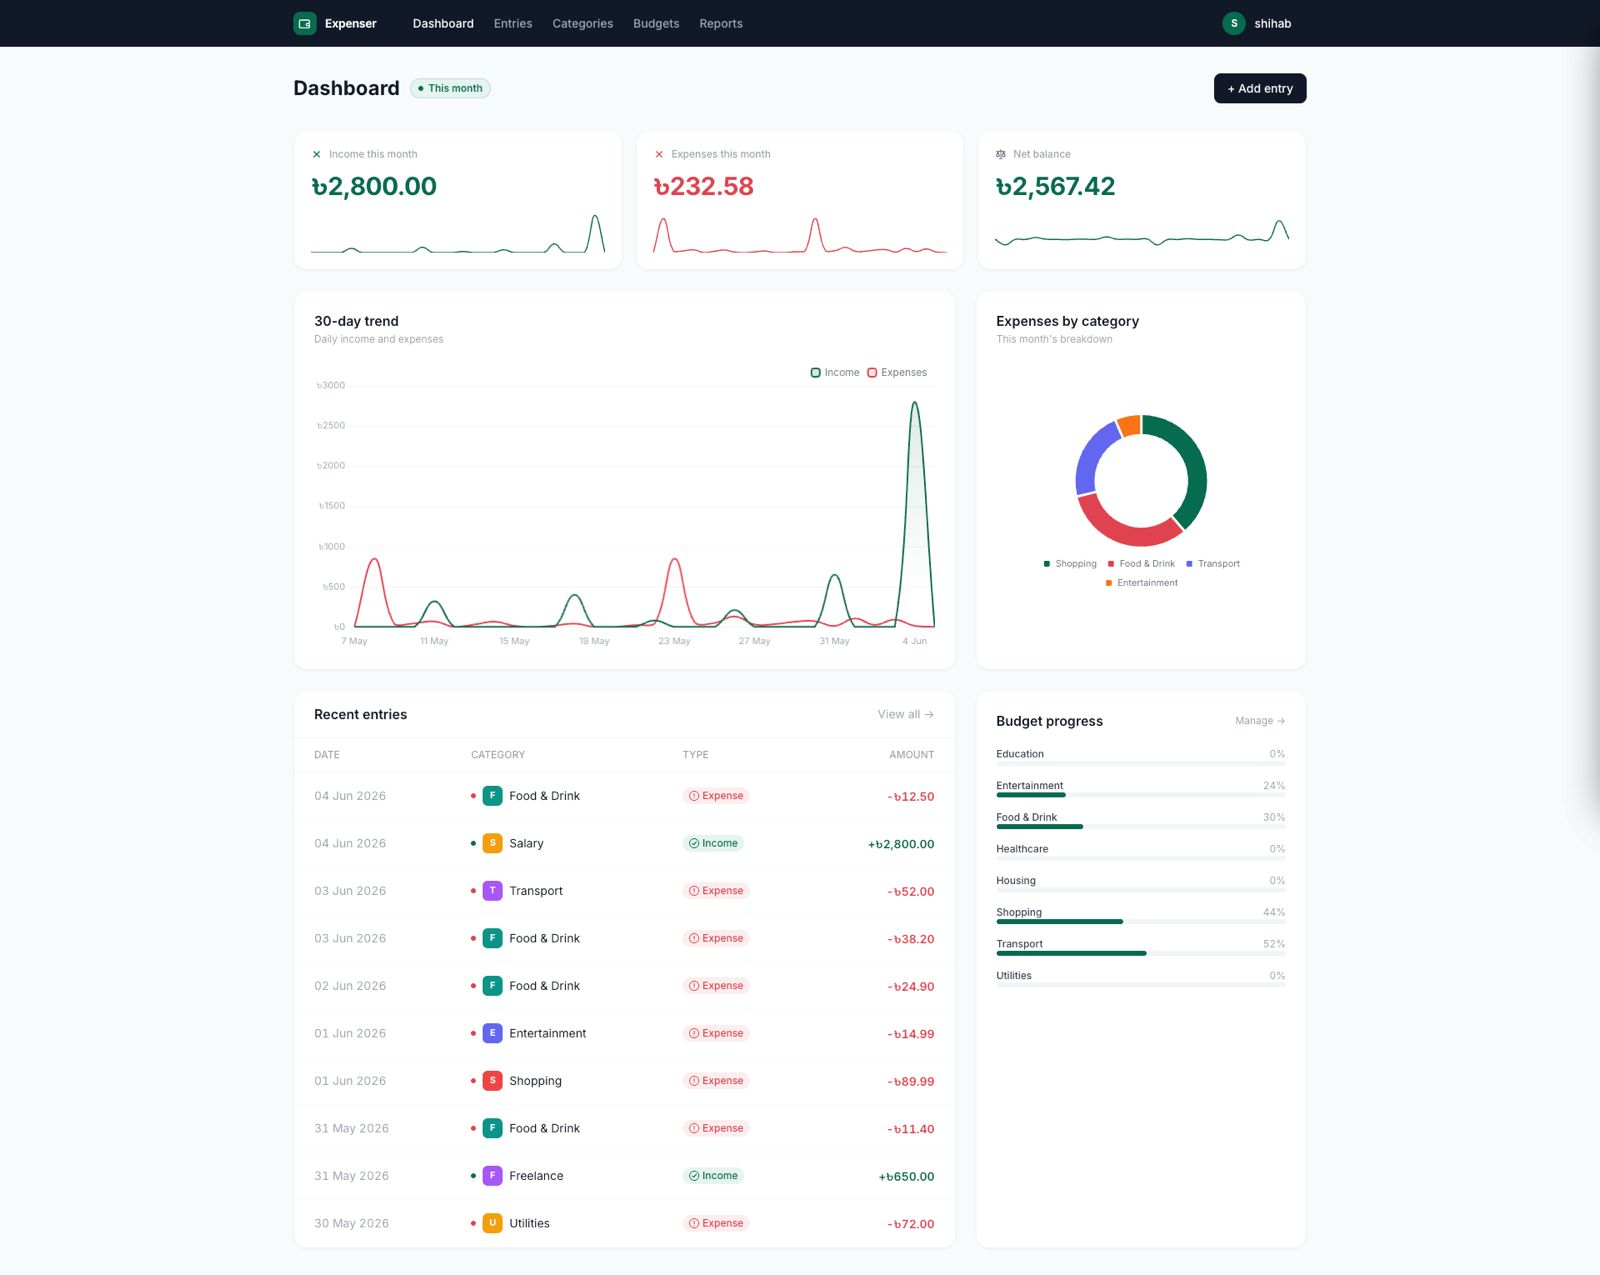
\includegraphics[width=\linewidth]{ss_dashboard.jpg}
\caption{Dashboard page}
\end{figure}

\section{Entries}

The entries page lists all transactions with filtering by type, category, tag, and date range. Each row shows the date, type badge, category avatar, description, and amount coloured green for income and red for expense.

\begin{figure}[htbp]
\centering
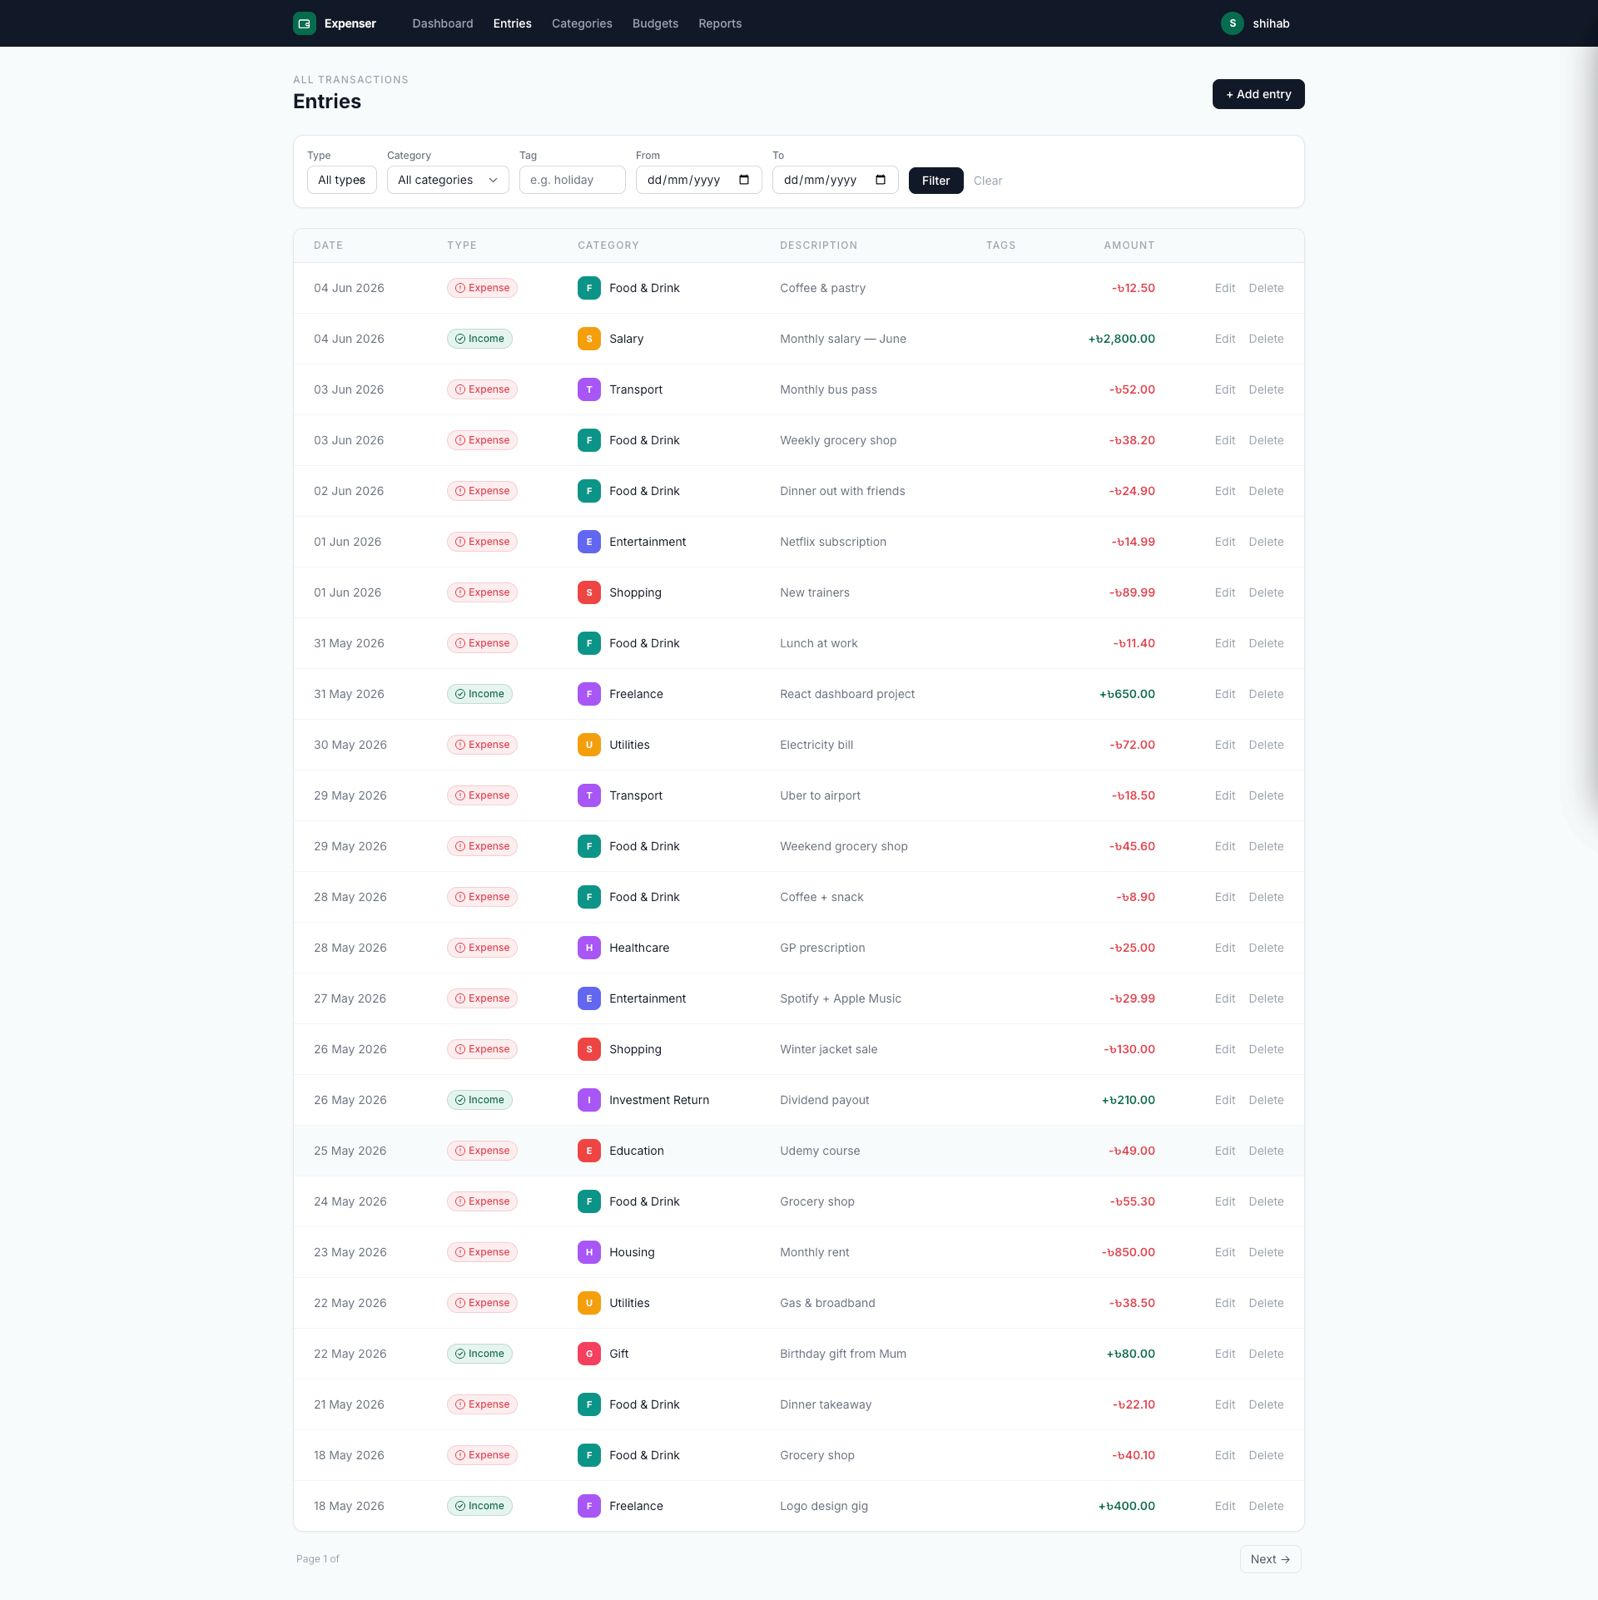
\includegraphics[width=\linewidth]{ss_entries.jpg}
\caption{Entries list page with filters}
\end{figure}

\section{Categories}

The categories page splits all categories into Income and Expense sections, each with a coloured letter avatar, type badge, and Edit/Delete actions.

\begin{figure}[htbp]
\centering
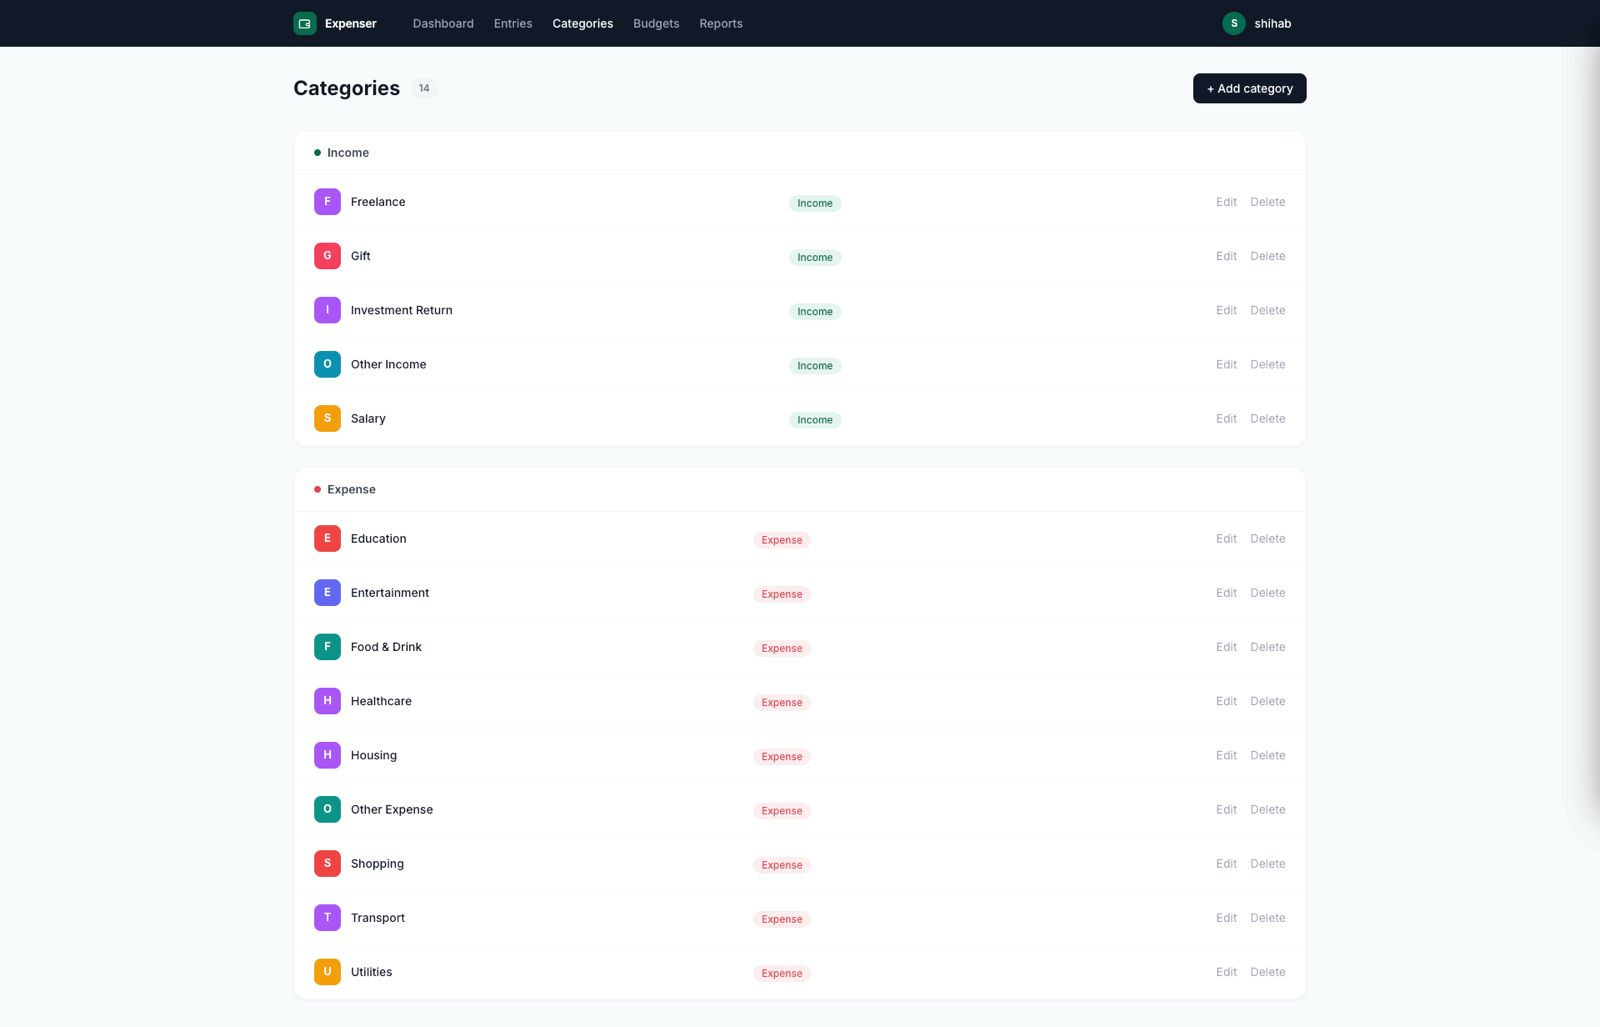
\includegraphics[width=\linewidth]{ss_categories.jpg}
\caption{Categories management page}
\end{figure}

\section{Budgets}

The budgets page shows each monthly budget with a progress bar indicating how much of the limit has been spent. The colour changes from green to amber at 80\% and red when the limit is exceeded.

\begin{figure}[htbp]
\centering
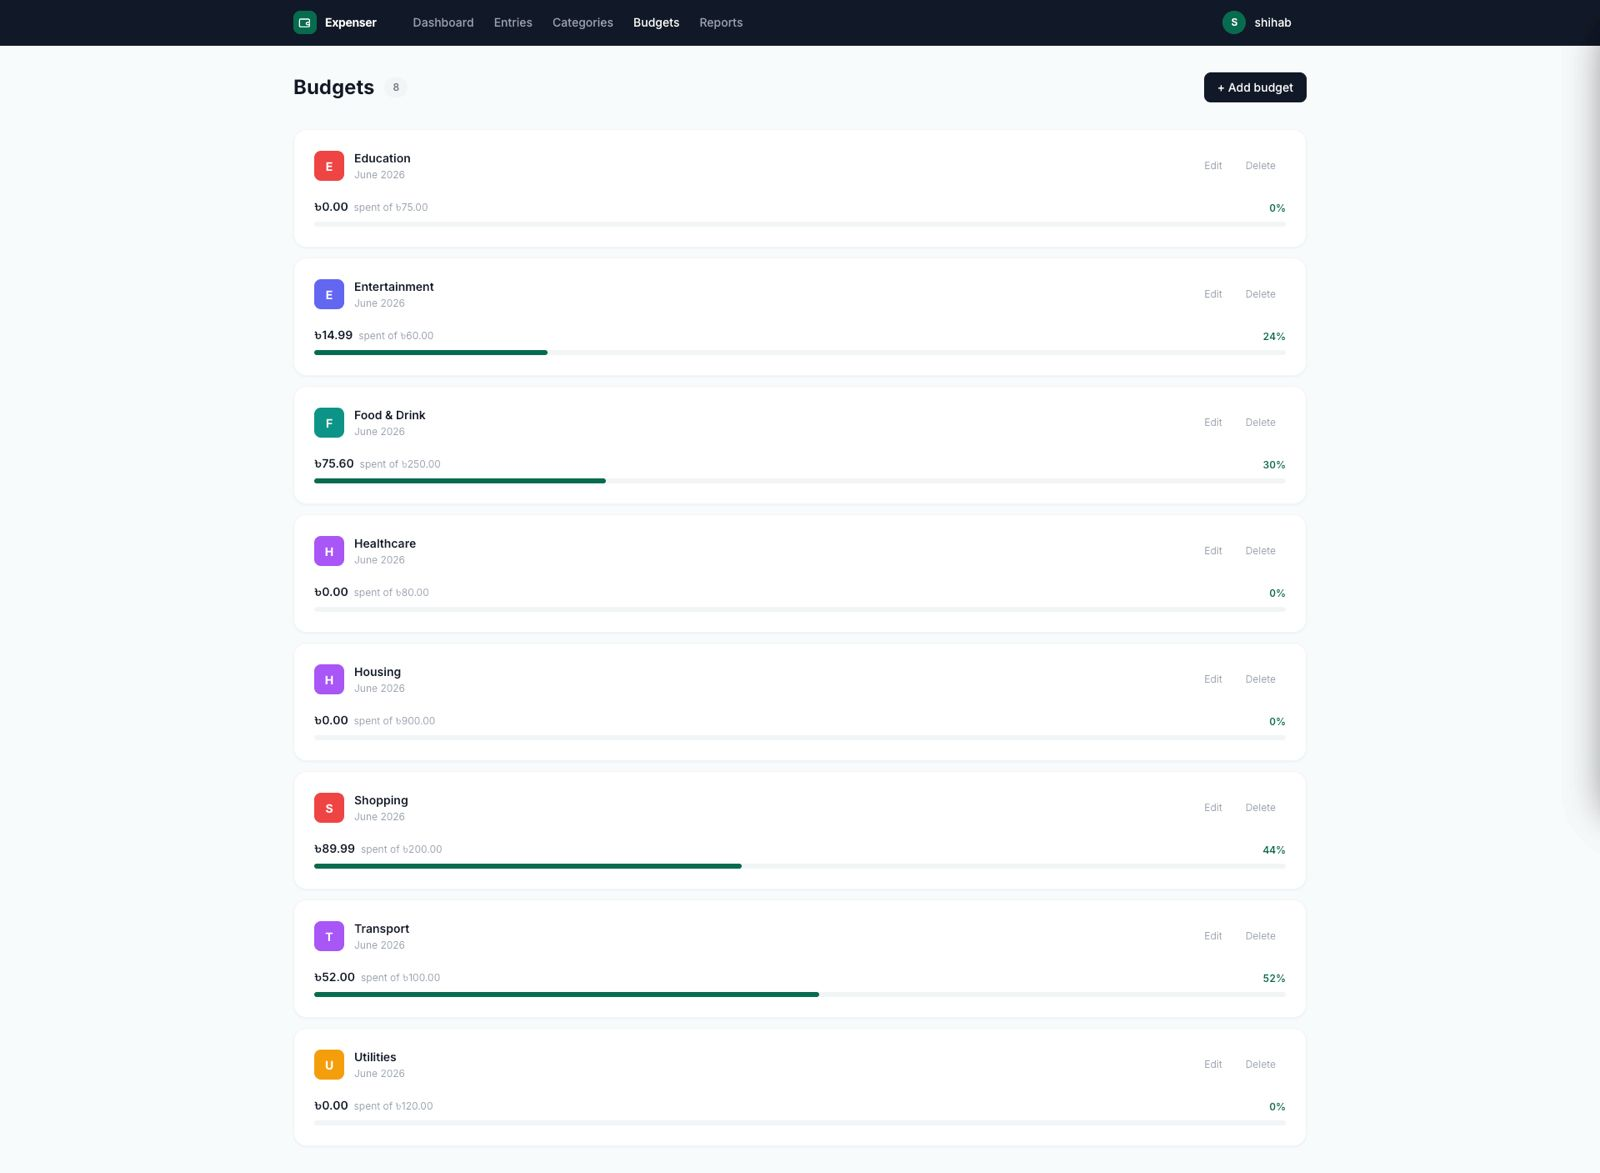
\includegraphics[width=\linewidth]{ss_budgets.jpg}
\caption{Budgets page with progress bars}
\end{figure}

\section{Reports}

The reports page allows selecting a date range preset and shows total income, expenses, and net balance for the period. A bar chart breaks down the top expense categories. Reports can be downloaded as a CSV file.

\begin{figure}[htbp]
\centering
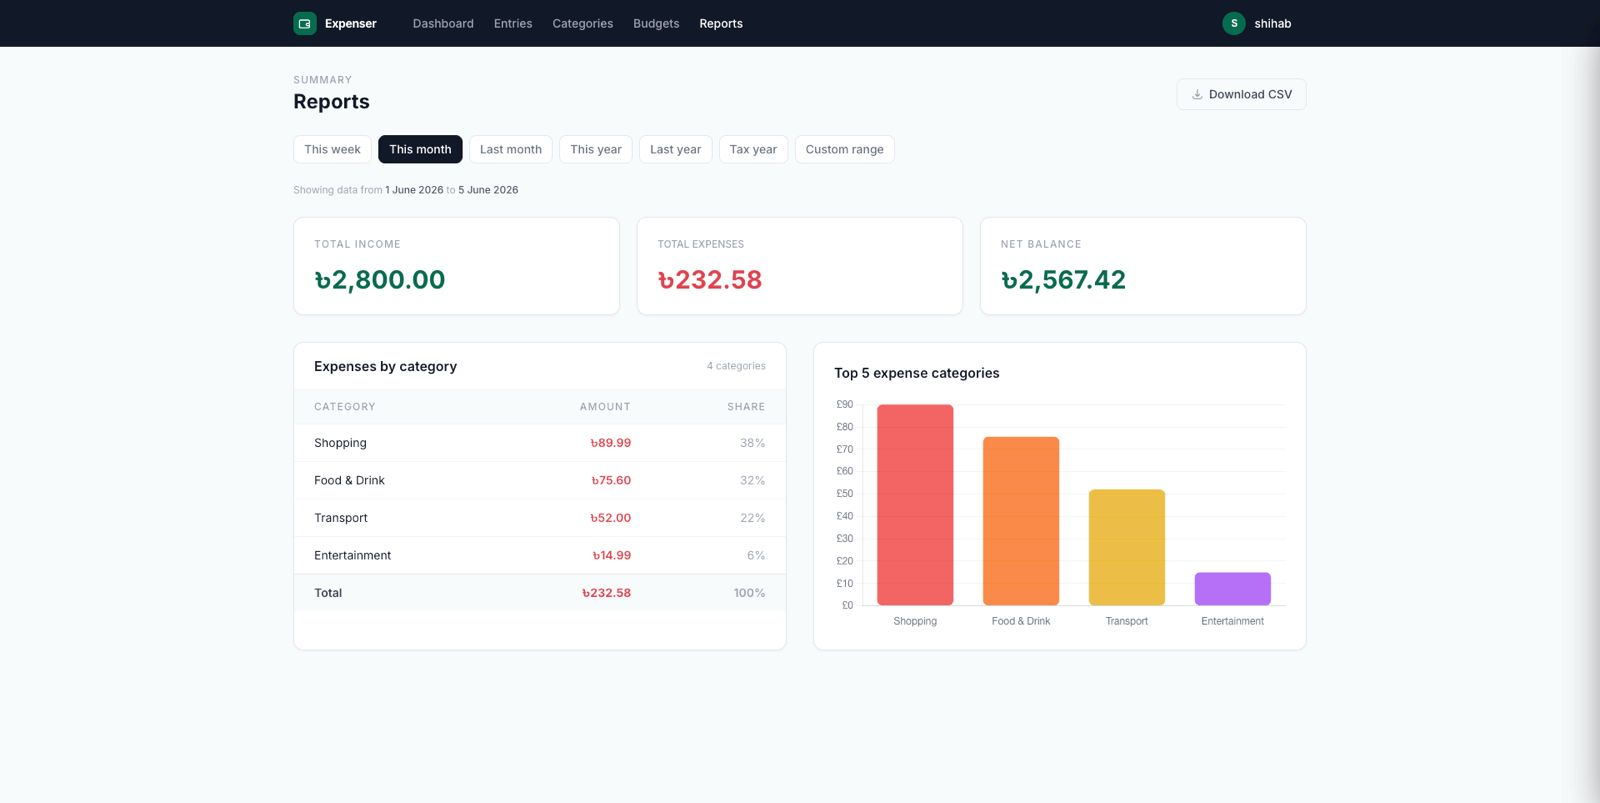
\includegraphics[width=\linewidth]{ss_reports.jpg}
\caption{Reports page with date range selector and bar chart}
\end{figure}

% ══════════════════════════════════════════════════════════════════════════════
\chapter{Future Work}
% ══════════════════════════════════════════════════════════════════════════════

The current version of Expenser covers all the core requirements of the project. However, there are several features we discussed during development that we did not have time to implement. These would be good additions in a future version:

\begin{itemize}[itemsep=5pt]
  \item \textbf{PDF report export} --- Currently reports can only be downloaded as CSV. Adding PDF export using a library like WeasyPrint would make the reports more presentable and easier to share.

  \item \textbf{Email notifications} --- The budget warning system currently only shows alerts on the page. It would be more useful to send an email to the user when they reach 80\% or exceed their budget limit for a category.

  \item \textbf{Automated recurring entry processing} --- The \texttt{process\_recurring} management command exists but has to be run manually. Scheduling it with a cron job on the Linux server would make recurring entries fully automatic.

  \item \textbf{Mobile responsive layout} --- The application works on desktop but the layout breaks on smaller screens. Improving the responsive design with Tailwind's mobile breakpoints would make it usable on phones.

  \item \textbf{User profile page} --- Currently users cannot change their username, email, or password from within the app. Adding a profile settings page would make account management easier.

  \item \textbf{Multi-currency support} --- Right now everything is in BDT. Allowing users to select their currency and optionally converting between currencies using an external API would make the app more internationally useful.

  \item \textbf{Automated tests} --- We did all our testing manually. Writing a proper test suite using \texttt{pytest-django} would make it easier to catch regressions when adding new features in the future.
\end{itemize}

% ══════════════════════════════════════════════════════════════════════════════
\chapter{Conclusion}
% ══════════════════════════════════════════════════════════════════════════════

We built Expenser as a working personal finance tracker using Django and PostgreSQL. The project helped us understand how to structure a real Django application with multiple apps, how to use class-based views properly, how forms and validation work, and how to use signals and custom management commands.

Working as a team through GitHub taught us how to manage branches, review each other's code, and merge work without breaking things. We ran into a few issues along the way, like resolving merge conflicts and debugging template rendering problems, but we sorted them out as we went.

The application covers all the core requirements: user authentication, transaction tracking, category and budget management, financial reports, and CSV export. It runs on a Linux virtual machine and the full setup process is documented in this report. The project gave us practical experience in team-based software development using Agile, which we think is the most valuable thing we took from this course.

\vspace{0.8cm}

\begin{center}
\begin{tabular}{@{}rl@{}}
\textbf{Git Repository:} & \url{https://github.com/shihabshaharia/expenser} \\[4pt]
\textbf{Access:}         & Public repository --- no credentials required \\
\end{tabular}
\end{center}

\begin{thebibliography}{9}
\bibitem{django} Django Software Foundation, \textit{Django Documentation}, version 5.2. \url{https://docs.djangoproject.com}
\bibitem{postgres} PostgreSQL Global Development Group, \textit{PostgreSQL Documentation}. \url{https://www.postgresql.org/docs}
\bibitem{tailwind} Tailwind Labs, \textit{Tailwind CSS Docs}. \url{https://tailwindcss.com/docs}
\bibitem{chartjs} Chart.js Contributors, \textit{Chart.js Docs}. \url{https://www.chartjs.org/docs}
\end{thebibliography}

\end{document}
